\begin{frame}{Two Regimes: Dense Clusters and Sparse Tails}
    \begin{columns}[T,onlytextwidth]
        \column{0.48\textwidth}
        \textbf{Dense cluster} ($U' = k_{\max} - k_{\min} \ll 2^L$)
        \smallskip
        \begin{itemize}\setlength{\itemsep}{0.35em}
            \item ARE (Goswami): $\;n\log_2(\mathcal{L}/\varepsilon)\;$ bits
                  --- \textbf{independent of $U$}
            \item ERE: $\;n\log_2(U'/n) + O(n)\;$ bits
                  --- \textbf{shrinks with $U'$}
        \end{itemize}
        \medskip
        \begin{center}
            \fbox{$\;U' \le n\mathcal{L}/\varepsilon
                    \;\Longrightarrow\; \text{exact mode,}\ \mathrm{FPR} = 0\;$}
        \end{center}

        \column{0.48\textwidth}
        \textbf{Sparse tail} (wide $U'$, few keys)
        \smallskip
        \begin{center}
            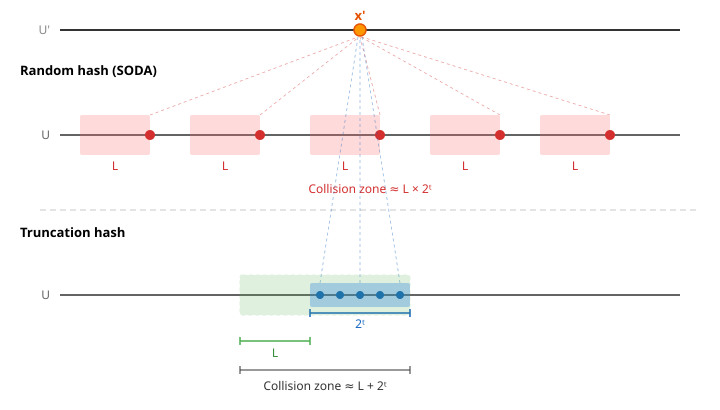
\includegraphics[width=0.92\linewidth, keepaspectratio]{../../figures/phantom_comparison_slide}
        \end{center}
        \begin{itemize}\setlength{\itemsep}{0.2em}
            \item SODA hash:\quad $\log_2(\mathcal{L}/\varepsilon)$ BPK
            \item Truncation:\quad $\log_2(1/\varepsilon)$ BPK
        \end{itemize}
    \end{columns}
\end{frame}
